\begin{fact}\label{iso-tri}
	Considérons tous les triangles de périmètre fixé $p$. Parmi tous ces triangles, celui d'aire maximale est le triangle équilatéral de côté $c = \dfrac13 p$.
\end{fact}


% ----------------------- %


\begin{proof}
	Soit un triangle $ABC$ non équilatéral, de sorte que $ABC$ n'est pas isocèle en $A$.
	Selon le fait \ref{iso-tri}, il existe un triangle isocèle de base $[BC]$, de même périmètre et d'aire strictement plus grande.
	Ceci nous prouve qu'un triangle non équilatéral ne peut pas être solution du problème, et par conséquent seul le triangle équilatéral maximise l'aire à périmètre fixé. Que c'est efficace!
\end{proof}


% ----------------------- %


\begin{remark}
	Voici un fait rigolo. Une application itérative du fait \ref{iso-tri} donne à la limite le triangle équilatéral d'aire maximale, et ceci avec une vitesse de convergence exponentielle.
	%
	En effet, partons d'un triangle $ABC$ quelconque de périmètre $p$, le fait \ref{iso-tri} nous donne successivement les triangles $ACD$, $ADE$ et $AEF$ isocèles en $D$, $E$ et $F$ respectivement, ayant tous pour périmètre $p$, et ceci avec des aires de plus en plus grandes.  
	Le dessin suivant amène à conjecturer qu'en poursuivant le procédé pour avoir ensuite un triangle $AFG$ isocèle en $G$...\,, nous aboutirons \og \emph{à la limite} \fg\ à un triangle équilatéral.

	\begin{center}
		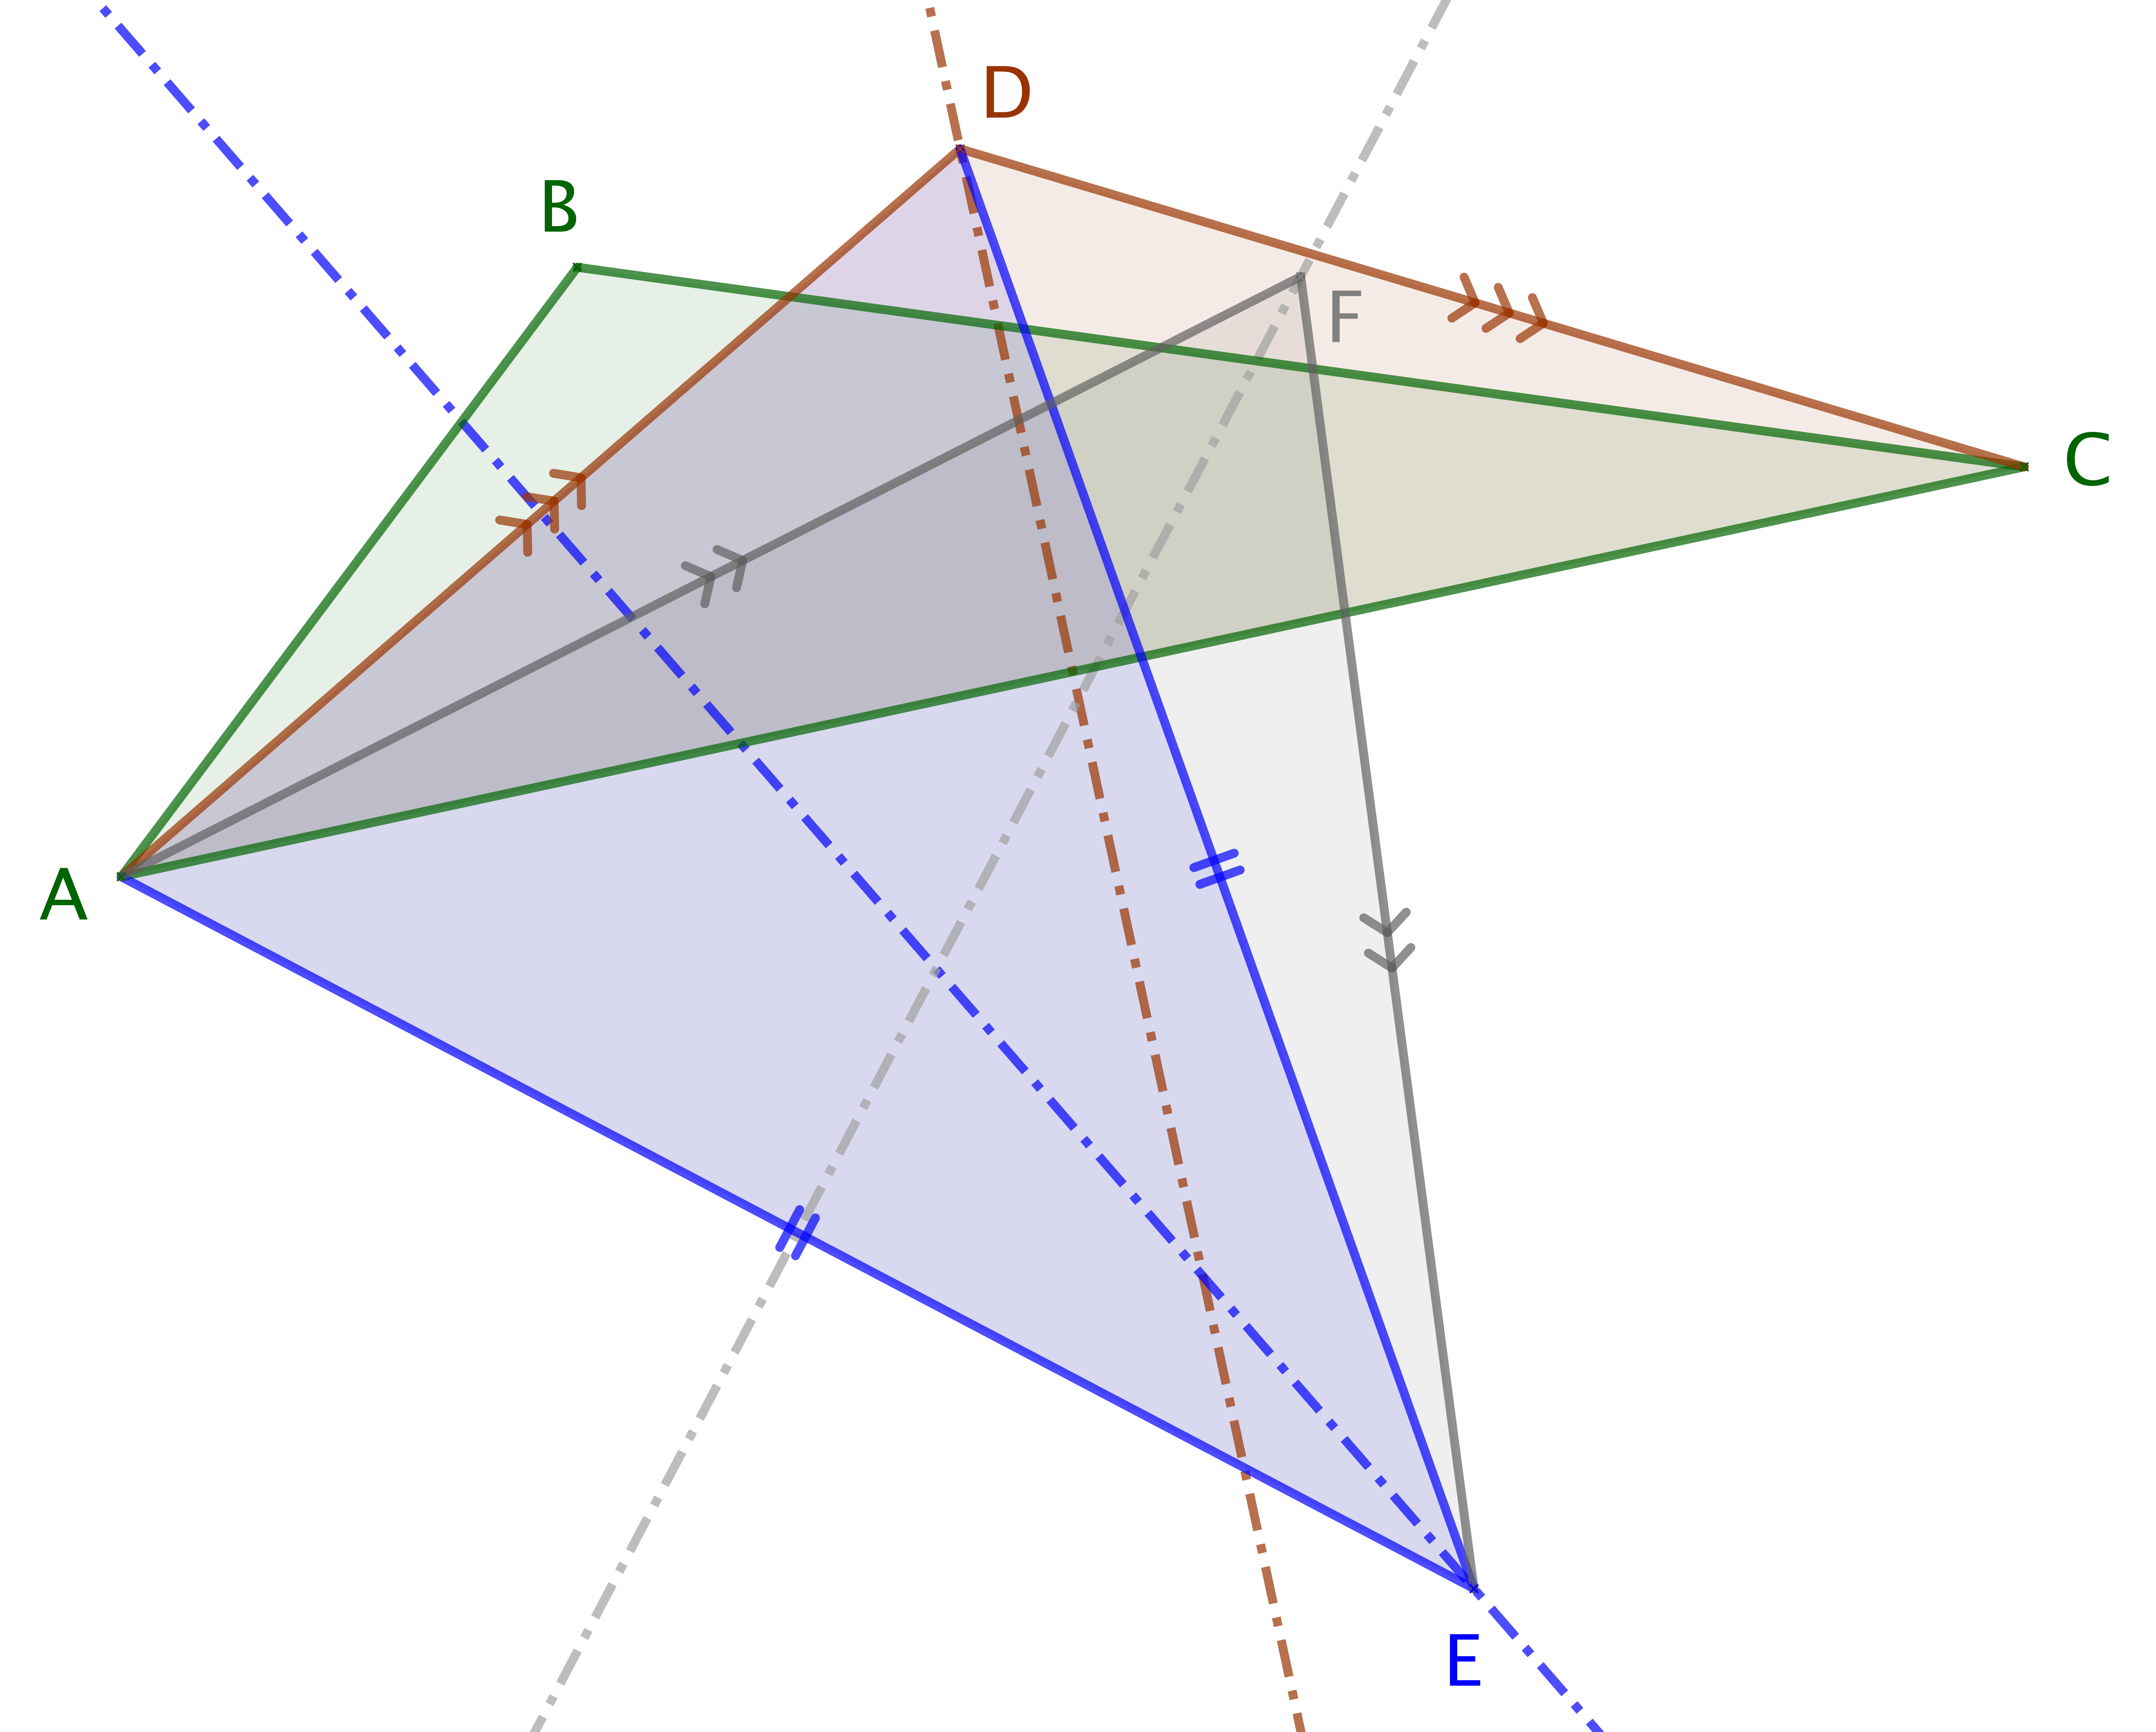
\includegraphics[scale=.4]{content/triangle-gene/triangle-conj.png}
	\end{center} 

	
	Le passage d'un triangle quelconque $ABC$ au triangle $ACD$ isocèle en $D$ nous amène à nous concentrer sur ce que donne notre procédé d'agrandissement d'aire à périmètre fixé pour des triangles isocèles. 
	Dans la suite, nous allons nous appuyer sur le schéma suivant.
	
	\begin{center}
		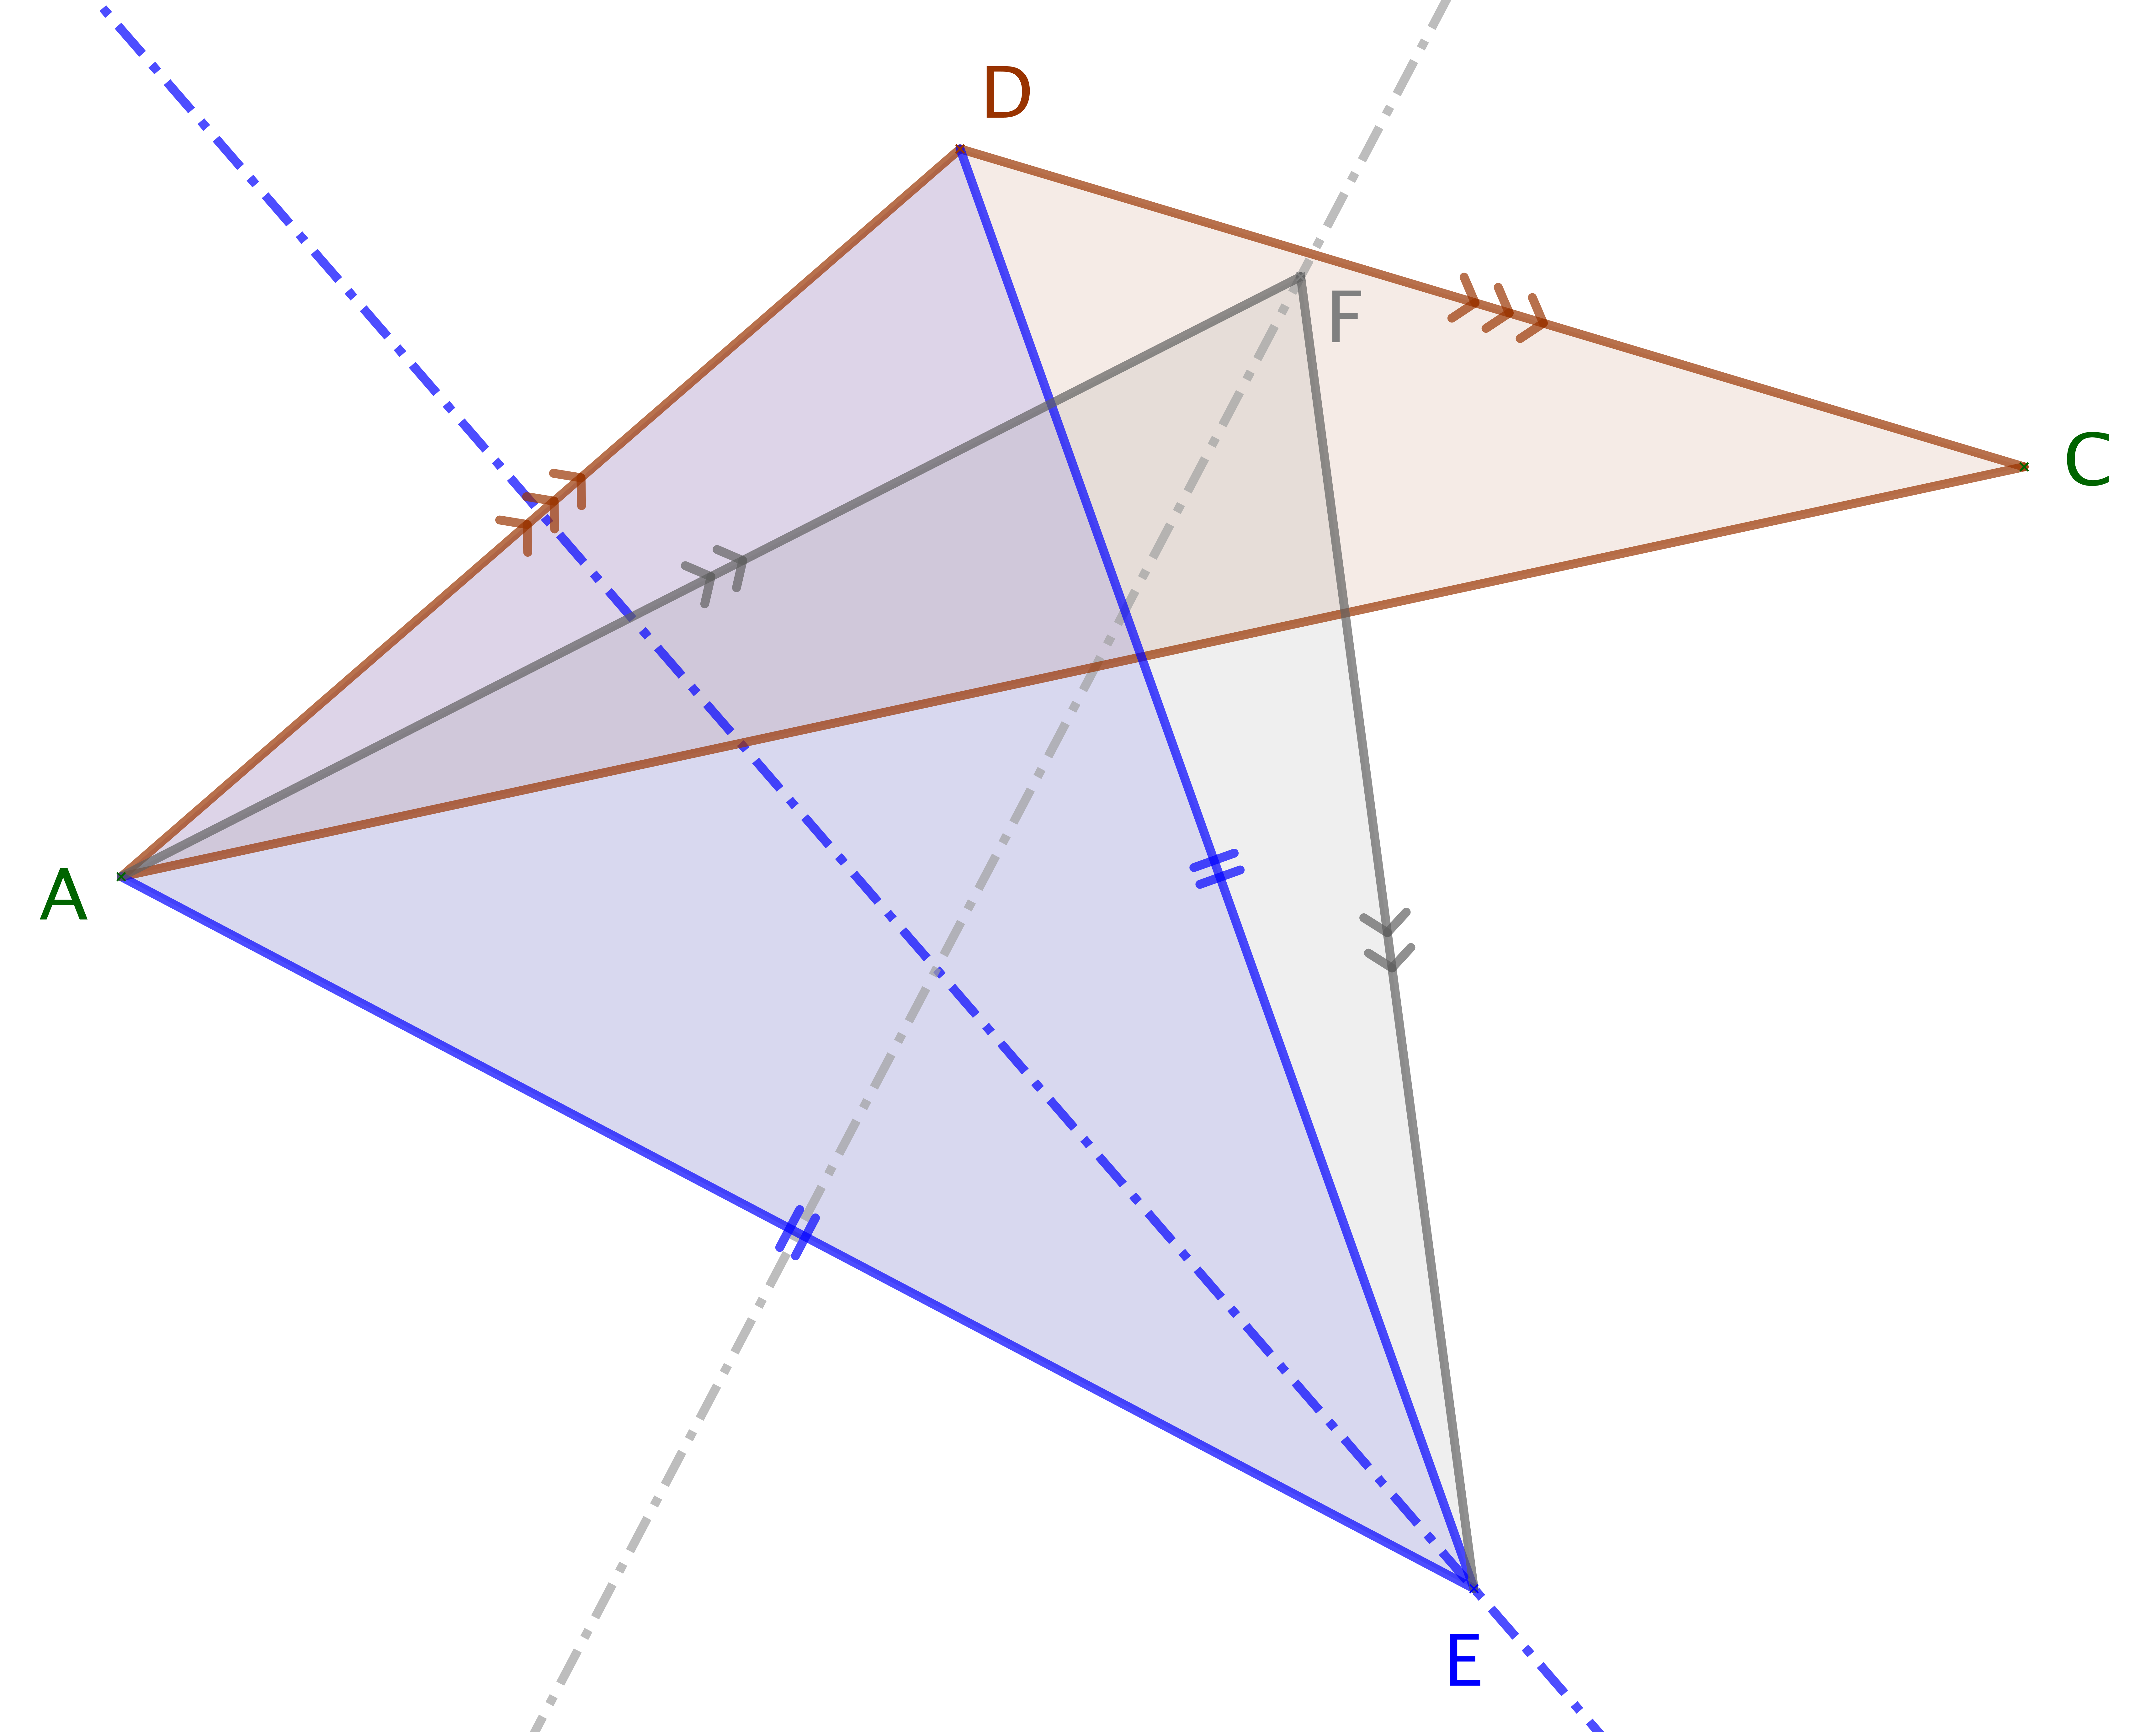
\includegraphics[scale=.4]{content/triangle-gene/triangle-proof.png}
	\end{center} 
	
	
	Voici ce que nous pouvons affirmer.
	%
	\begin{enumerate}
		\item Considérons $ACD$ isocèle en $D$ tel que $AC > AD$.
		%
		Comme $AC + AD + DC = p$, nous avons $AC > \frac13p > AD$.
		Dès lors, on doit avoir ensuite  $AD < \frac13p < AE$, car $AD + DE + AE = p$ et $AD = AE$.


		\item Considérons $ADE$ isocèle en $E$ tel que $AD < AE$ en oubliant le point précédent.
		%
		Comme $AD + DE + AE = p$, nous avons $AD < \frac13p < AE$.
		Dès lors, on doit avoir ensuite  $AE > \frac13p > AF$, car $AE + AF + EF = p$ et $AF = EF$.


		\item Les deux points précédents démontrent que notre procédé n'arrivera jamais en un nombre fini d'étapes à un triangle équilatéral si l'on part d'un triangle isocèle non équilatéral.%
		\footnote{
			Et plus généralement si le procédé ne commence pas avec une base de longueur $\frac13 p$.
		}


		\item Nous devons quantifier les écarts à la mesure \og \emph{limite} \fg\ $p^{\,\prime} = \frac13 p$. 
		%
		\begin{itemize}
			\item Dans $ADC$, posant $AD = p^{\,\prime} - \epsilon$, nous avons $AC = p^{\,\prime} + 2 \epsilon$.

			\item Dans $ADE$, posant $AE = p^{\,\prime} + \epsilon^{\,\prime}$, nous avons $AD = p^{\,\prime} - 2 \epsilon^{\,\prime}$.

			\item Donc $\epsilon^{\,\prime} = \dfrac12 \epsilon$.
		\end{itemize}
		
		\noindent
		Nous avons donc une convergence exponentielle des longueurs des côtés vers $p^{\,\prime} = \frac13 p$. Et tout ceci via de la géométrie et de l'analyse élémentaires!
	\end{enumerate}
\end{remark}


% ----------------------- %


\begin{remark}
	La formule de Héron donne qu'un triangle de côtés $a$, $b$ et $c$, et de demi-périmètre $s = \num{.5} p$, possède une aire égale à $\sqrt{s(s - a)(s - b)(s - c)}$.
	La comparaison des moyennes géométriques et arithmétiques d'ordre $3$ nous donne alors une solution algébrique efficace, puisque 
	$\sqrt[3]{(s - a)(s - b)(s - c)} \leq \frac13 \big( (s - a) + (s - b) + (s - c) \big)$
	nous donne alors
	$s(s - a)(s - b)(s - c) \leq \frac{1}{27} s^4$,
	puis
	$\sqrt{s(s - a)(s - b)(s - c)} \leq \frac{p^2}{12 \sqrt{3}}$
	où $\frac{p^2}{12 \sqrt{3}}$ est l'aire du triangle équilatéral de périmètre $p$.
\end{remark}


% ----------------------- %


\begin{remark} \label{constrained-extrema}
	L'aire du triangle étudié étant de mesure positive ou nulle, nous cherchons à maximiser son carré
	$f(a;b;c) = s(s - a)(s - b)(s - c)
	          = \frac{1}{16} (a + b + c)(b + c - a)(a + c - b)(a + b - c)$,
	sous la contrainte $2s = a + b + c$ où $s > 0$ est constant.
	Notant $g(a;b;c) = a + b + c - 2 s$, la contrainte s'écrit $g(a;b;c) = 0$.
	Selon la méthode des extrema liés, un éventuel extremum doit vérifier 
	$\pder[i]{f}{a}{1} = \lambda \pder[i]{g}{a}{1}$,
	$\pder[i]{f}{b}{1} = \lambda \pder[i]{g}{b}{1}$ et
	$\pder[i]{f}{c}{1} = \lambda \pder[i]{g}{c}{1}$
	avec $\lambda \in \RR$ une constante.
	En particulier, nous obtenons
	$- s(s - b)(s - c) = - s(s - a)(s - c) = - s(s - a)(s - b)$,
	et par conséquent
	$(s - b)(s - c) = (s - a)(s - c) = (s - a)(s - b)$.
	Les cas $s = a$, $s = b$ et $s = c$ donnent $f(a;b;c) = 0$.
	Quant au cas $\big[ s \neq a, s \neq b \text{ et } s \neq c \big]$, il n'est envisageable que si $a = b = c = \frac{p}{3}$ qui implique $f(a;b;c) = \frac{1}{16} p \big( \frac{p}{3} \big)^3 = \big( \frac{p^2}{12 \sqrt{3}} \big)^2 > 0$.
	En résumé, l'existence d'un maximum implique que ce maximum corresponde au cas du triangle équilatéral.
	Il reste à démontrer qu'un tel maximum existe pour pouvoir conclure: ceci est facile à justifier en considérant l'ensemble compact $\intervalC{0}{2s}^3$ de $\RR^3$.
\end{remark}
